\documentclass[aps,prl,reprint,superscriptaddress,nofootinbib,floatfix]{revtex4-2}

\usepackage{amsmath}
\usepackage{amssymb}
\usepackage{graphicx}
\usepackage{hyperref}

\graphicspath{{../results/T2_NG15yr/figures/}}

\begin{document}

\title{Curved SMBHB Spectra Compete with New-Physics Explanations in PTA Source Identification}

\author{Ran DUAN}
\email{rduan@chenli.science}
\affiliation{chenli science}
\date{\today}

\begin{abstract}
The NANOGrav 15-year Hellings--Downs signal admits both astrophysical
and cosmological interpretations.  We test whether the published
new-physics Bayes factors remain discriminating once template
provenance, density construction, and curved-SMBHB controls are matched.
Official PTArcade templates and official PTArcade \texttt{ceffyl}
densities reproduce the published SIGW-Gaussian, SIGW-delta, and
cosmic-superstring log-Bayes factors at sub-nat agreement.  On that
calibrated scale, one environmental SMBHB model and two phenomenological
low-frequency curvature surrogates yield
$\ln\mathcal{B}=3.45$--$3.84$, all within one nat of the leading
cosmological templates.  The $0.681$-nat gap between the leading
SIGW-Gaussian model and the best curved-SMBHB control is comparable to the
identified calibration and prior-boundary systematics.  Current data
therefore do not yet support robust source discrimination between
leading cosmological stochastic spectra and curved SMBHB explanations.
\end{abstract}

\maketitle

\emph{Introduction.}
Pulsar timing arrays have opened the nanohertz gravitational-wave
window.  The NANOGrav 15-year data set reports a common red process with
Hellings--Downs spatial correlations \cite{NANOGrav_15yr_GWB}.  The
companion noise analysis \cite{NANOGrav_15yr_noise} provides the
white-noise budget used in the public analyses.  The signal is
compatible with an astrophysical supermassive-black-hole-binary (SMBHB)
background \cite{Phinney_2001} and with several cosmological sources.
The NANOGrav
new-physics search \cite{NANOGrav_15yr_NewPhysics}, using PTArcade
\cite{PTArcade_2023}, reports strong-but-not-decisive Bayes factors
relative to the SMBHB baseline for several leading stochastic
alternatives, including SIGW-Gaussian ($\mathcal{B}=57$), SIGW-delta
($\mathcal{B}=44$), and cosmic superstrings ($\mathcal{B}=46$),
placing these models in the strong-but-not-decisive evidence range
under the Kass--Raftery convention \cite{Kass_Raftery_1995}.
We show below that one environmental SMBHB model and two phenomenological
curved-SMBHB surrogates are competitive with these alternatives on the
same evidence scale.

The central issue is reproducibility of Bayesian source identification.
Order-unity shifts in $\ln\mathcal{B}$ can arise from the
scalar-induced-gravitational-wave kernel, the radiation-era resonance,
prior boundaries on peak frequency, or the density estimate used for the
free-spectrum likelihood \cite{Kohri_Terada_2018}.  We therefore
separate three questions: whether our PTA pipeline reproduces the
published Hellings--Downs posterior, whether a local spectral library
reproduces the qualitative model ranking, and whether the official
PTArcade spectra plus official density products reproduce the published
absolute Bayes factors.

\emph{Templates and likelihood.}
We model an isotropic stochastic background through the one-sided strain
power spectral density $S_h(f)$ and
\begin{equation}
\Omega_\mathrm{GW}(f)=\frac{2\pi^2}{3H_0^2} f^3 S_h(f),
\end{equation}
with $H_0=67.4\,\mathrm{km\,s^{-1}\,Mpc^{-1}}$.  The template library
includes SMBHB power laws, SMBHB environmental hardening
\cite{Sesana_2013,Sampson_2015},
SIGW-Gaussian, SIGW-delta, stable Nambu--Goto strings, cosmic
superstrings, and two first-order phase-transition spectra.  All
$\Omega_\mathrm{GW}$ calculations are dimension-checked in
\texttt{code/gwb\_templates.py}.

For the PTA likelihood we use ENTERPRISE \cite{ENTERPRISE_2019}.
White-noise parameters EFAC, EQUAD, and ECORR are fixed to the official
NANOGrav 15-year noise dictionary \cite{NANOGrav_15yr_noise}.  The
common process uses 14 GWB Fourier bins at $f_i=i/T$, matching the
NANOGrav low-frequency truncation \cite{NANOGrav_15yr_GWB,
NANOGrav_15yr_NewPhysics}.  Timing-model offsets are marginalized with
\texttt{MarginalizingTimingModel}; timing-model files are not modified.
Model evidences are computed either from local free-spectrum KDE
products or from the official PTArcade \texttt{ceffyl} density grid
using \texttt{dynesty} nested sampling \cite{Speagle_2020}.

\emph{Pipeline validation.}
Direct ingestion of the pre-sampled NANOGrav Hellings--Downs chain gives
$\log_{10}A_\mathrm{HD,vg}=-14.20\pm0.13$ and
$\gamma=3.25\pm0.35$, matching the published result
\cite{NANOGrav_15yr_GWB}.  Our independent
$2\times10^6$-step Hellings--Downs PTMCMC chain
\cite{PTMCMCSampler_2017} gives
\begin{equation}
\begin{aligned}
\log_{10}A_\mathrm{GWB}&=-14.199\pm0.122,\\
\gamma_\mathrm{GWB}&=3.272\pm0.321 .
\end{aligned}
\end{equation}
A second $5\times10^5$-step chain initialized from dispersed cold
conditions converges to $\log_{10}A=-14.251\pm0.168$ and
$\gamma=3.401\pm0.418$.  Tail-aligned warm+cold segments yield
$\hat R(\log_{10}A)=1.047$ and $\hat R(\gamma)=1.047$, below an
a priori convergence threshold of $1.05$.  A third hot-chain attempt was
rejected because it remained at $-\infty$ posterior metadata with zero
accepted jumps.

\begin{figure}[t]
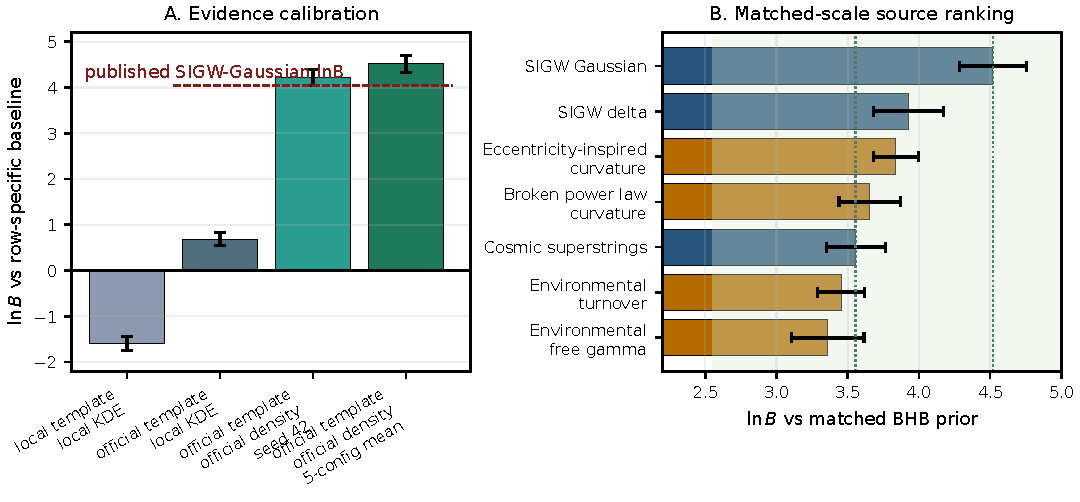
\includegraphics[width=\columnwidth]{prl_decisive_evidence_figure.pdf}
\caption{\label{fig:evidence}
Evidence calibration and matched-scale source ranking.  Panel A shows
that neither a local template/local-density refit nor an official
template with a local KDE reproduces the SIGW-Gaussian absolute Bayes
factor.  The first Panel-A bar uses a fixed-$\gamma$ SMBHB baseline; the
remaining Panel-A bars and all Panel-B models use the PTArcade BHB-prior
baseline.  The horizontal reference line marks the published
PTArcade-baseline SIGW-Gaussian value and applies only to the last three
bars.  Panel B compares leading cosmological templates (blue) with
curved-SMBHB controls (orange) on the matched evidence scale.}
\end{figure}

\emph{Evidence calibration.}
Our local \texttt{ceffyl}-style refit starts from the released
Hellings--Downs 30-bin free-spectrum core, builds independent per-bin
KDEs for the 14 lowest bins, and evaluates each spectral template
through
\begin{equation}
\ln\mathcal{L}(\theta)=
\sum_{k=1}^{14}
\ln\mathrm{KDE}_k[\log_{10}\rho_k^\mathrm{model}(\theta)] .
\end{equation}
This local refit reproduces the qualitative NANOGrav ranking but not
the published absolute values.  Sensitivity sweeps show that KDE
bandwidth, not nested-sampler seed or live-point count, dominates the
local-refit uncertainty.

We then isolate the source of the discrepancy.  The released
Hellings--Downs free-spectrum covariance is nearly diagonal: max
$|\mathrm{corr}_{ij}|=0.227$, mean $|\mathrm{corr}_{ij}|=0.030$, and
effective rank $13.56/14$.  A covariance-aware projection gives a
negligible correction for SIGW-Gaussian versus SMBHB,
$\Delta\ln\mathcal{Z}\simeq -0.006$ nat, and a modest correction for the
poor flat-string proxy, $\simeq+1.31$ nat.  Covariance restoration
therefore cannot explain a multi-nat absolute-Bayes-factor gap.

The decisive test uses the official NANOGrav/PTArcade model files and
the official PTArcade \texttt{ceffyl} density product.  PTArcade model
files return $h^2\Omega_\mathrm{GW}$, so the residual conversion is
\begin{equation}
\rho^2=\frac{(H_0/h)^2\,h^2\Omega_\mathrm{GW}}
{8\pi^4 f^5 T}.
\end{equation}
This conversion was checked against \texttt{ptarcade.models\_utils.
omega2cross} to relative precision below $5\times10^{-16}$.

\begin{table}[t]
\caption{\label{tab:lnb}
Official-density Bayes factors relative to the PTArcade BHB-prior
baseline.  The first three rows are five-configuration means used to
calibrate the published NANOGrav values; the last three rows are
five-configuration means for the best-performing tested representative
of each curved-SMBHB class.}
\begin{ruledtabular}
\begin{tabular}{@{}lcc@{}}
Model & $\ln\mathcal{B}$ & Note \\
\hline
SIGW-Gaussian & $4.520\pm0.185$ & $\Delta_\mathrm{pub}=+0.477$ \\
SIGW-delta & $3.930\pm0.199$ & $\Delta_\mathrm{pub}=+0.146$ \\
Superstrings & $3.558\pm0.145$ & $\Delta_\mathrm{pub}=-0.271$ \\
Ecc.-curved SMBHB & $3.839\pm0.043$ & best tested repr. \\
Broken-PL SMBHB & $3.656\pm0.154$ & best tested repr. \\
Env. SMBHB & $3.453\pm0.062$ & best tested repr. \\
\end{tabular}
\end{ruledtabular}
\end{table}

Figure~\ref{fig:evidence} and Table~\ref{tab:lnb} show sub-nat
official-density reproduction for the three published cosmological
templates; the largest absolute residual across the five configurations
is $0.694$ nat for SIGW-Gaussian.  In contrast, replacing only the
SIGW-Gaussian spectrum while retaining the local scipy-KDE density gives
$\ln\mathcal{B}=+0.687\pm0.147$, still low by $3.36$ nats.  Absolute
evidence alignment is therefore controlled primarily by official density
construction and template fidelity, not by bin covariance.

The same matched evidence scale changes the physical interpretation.
Curved-SMBHB controls are not a single-model accident:
eccentricity-inspired, smooth broken-power-law, and environmental
turnover parameterizations give five-configuration means
$3.839\pm0.043$, $3.656\pm0.154$, and $3.453\pm0.062$,
respectively.  The best curved-SMBHB model lies only $0.681$ nat below
SIGW-Gaussian and $0.091$ nat below SIGW-delta, and exceeds the
superstring mean.  The $0.681$-nat gap between the leading
SIGW-Gaussian model and the best curved-SMBHB control is comparable to the
identified calibration and prior-boundary systematics, so it should not
be interpreted as robust source discrimination.  Independent prior-space
Sobol thermodynamic integration agrees with the dynesty robust means to
within $0.12$ nat for the leading cosmological templates and within
$0.063$ nat for the tested curved-SMBHB representatives.

The Supplemental Material gives the full official-density stochastic-model
ranking, curved-SMBHB family table, prior-boundary tests, and cumulative
low-frequency-bin scan.  In the single-configuration official scan the
leading six stochastic templates are SIGW-Gaussian, SIGW-delta, SIGW-box,
cosmic superstrings, metastable strings, and domain walls.  Extending the
SIGW-delta upper prior from $\log_{10}f_\mathrm{peak}\le -5$ to $-3$
increases its evidence by $0.426$ nat, a modest but non-negligible
boundary systematic.  Cumulative-bin evidence shows that SIGW-delta,
cosmic superstrings, eccentricity-inspired curvature, and environmental
turnover are already within $0.5$ nat of their 14-bin values by the
lowest eight Fourier bins, whereas SIGW-Gaussian and broken-power-law
curvature require ten bins.

\emph{Interpretation and conclusions.}
The NANOGrav 15-year data do not yet identify the physical origin of the
background.  On a calibrated evidence scale, current leading
new-physics preferences are compressed into the same model-comparison
tier as curved SMBHB spectra.  The sharpest near-term
discriminant is spectral shape at low frequency: SMBHBs give
$h^2\Omega_\mathrm{GW}\propto f^{2/3}$, while causal cosmological
sources such as SIGW and first-order phase transitions rise as $f^3$
below their characteristic scale \cite{Caprini_Figueroa_2018}.  Our
cumulative-bin scan makes this quantitative: the lowest eight to ten
Fourier bins already determine the matched-scale ranking to within
$0.5$ nat for the leading stochastic templates.

The practical lesson is physical as well as methodological.  A local
free-spectrum KDE product is useful for fast diagnostics, but it is not
automatically equivalent to the official PTArcade \texttt{ceffyl}
density.  For absolute Bayes factors at the sub-nat level, the official
density product, exact template implementation, and matched SMBHB prior
baseline must be used together.  More importantly, cosmological
alternatives should not be interpreted as source identification until
they are calibrated against curved SMBHB controls.  On the calibrated
evidence scale, three distinct curved-SMBHB parameterizations occupy the
same model-comparison tier as the leading cosmological stochastic
templates.  The remaining evidence gap is comparable to the calibration
and prior-boundary systematics identified here, so the present NANOGrav
15-year data do not yet support robust source identification among these
leading stochastic explanations.  CAR/bin covariance is a useful
diagnostic but is not the
dominant error budget for the leading SIGW/string comparisons.  This
claim is restricted to stochastic spectral-template comparisons
evaluable on the released free-spectrum density; time-domain PBH and
ULDM signal classes require their own likelihood objects.

\section*{Data and Code Availability}

The analysis uses public NANOGrav 15-year data products
\cite{NANOGrav_15yr_GWB,NANOGrav_15yr_noise}, official
NANOGrav/PTArcade model files from Zenodo DOI
\href{https://doi.org/10.5281/zenodo.8084351}{10.5281/zenodo.8084351},
and the official PTArcade \texttt{ceffyl} density product from Zenodo
DOI \href{https://doi.org/10.5281/zenodo.10495907}
{10.5281/zenodo.10495907}.  The code and compact data release corresponding
to this submission is mirrored at
\href{https://github.com/duan0004/paperdata}
{\texttt{github.com/duan0004/paperdata}} at commit
\texttt{4d3972e11a24ffee026a8e2214eb12dd19fbc2ea}.  Local checksums and
reproduction commands are recorded in \texttt{REPRODUCIBILITY.md}.

\begin{thebibliography}{13}

\bibitem{NANOGrav_15yr_GWB}
G. Agazie et al. (NANOGrav Collaboration), arXiv:2306.16213.

\bibitem{NANOGrav_15yr_noise}
G. Agazie et al. (NANOGrav Collaboration), arXiv:2306.16214.

\bibitem{NANOGrav_15yr_NewPhysics}
A. Afzal et al. (NANOGrav Collaboration), arXiv:2306.16219.

\bibitem{PTArcade_2023}
A. Mitridate et al., arXiv:2306.16377.

\bibitem{Phinney_2001}
E. S. Phinney, astro-ph/0108028.

\bibitem{Sesana_2013}
A. Sesana, Mon. Not. R. Astron. Soc. 433, L1 (2013),
arXiv:1211.5375.

\bibitem{Sampson_2015}
L. Sampson, N. J. Cornish, and S. T. McWilliams, Phys. Rev. D 91,
084055 (2015), arXiv:1505.07179.

\bibitem{Kass_Raftery_1995}
R. E. Kass and A. E. Raftery, J. Am. Stat. Assoc. 90, 773 (1995).

\bibitem{ENTERPRISE_2019}
J. A. Ellis et al., Zenodo 4059815 (2019).

\bibitem{PTMCMCSampler_2017}
J. A. Ellis and R. van Haasteren, Zenodo 1037579 (2017).

\bibitem{Speagle_2020}
J. S. Speagle, Mon. Not. R. Astron. Soc. 493, 3132 (2020),
arXiv:1904.02180.

\bibitem{Kohri_Terada_2018}
K. Kohri and T. Terada, Phys. Rev. D 97, 123532 (2018),
arXiv:1804.08577.

\bibitem{Caprini_Figueroa_2018}
C. Caprini and D. G. Figueroa, Class. Quantum Grav. 35, 163001 (2018),
arXiv:1801.04268.

\end{thebibliography}

\end{document}
